\documentclass{article}
\usepackage{biblatex}
\addbibresource{reference.bib}
\usepackage{graphicx} % Required for inserting images
\usepackage{geometry}
\usepackage{amsmath}
\usepackage{url}
\usepackage{float}
\usepackage{xcolor}
\usepackage{listings}
\usepackage{caption}
\usepackage{subcaption}
\usepackage{xparse}
\usepackage{hyperref}
\usepackage{amssymb}
\usepackage{verbatim}
\usepackage{fancyhdr}
\pagestyle{fancy}
\usepackage{xspace}
\cfoot{}
\lfoot{Università degli Studi di Padova, Laboratorio di Microelettronica, AA 2022-2023}
\rfoot{\thepage}

\title{Esperienza di laboratorio\\\textbf{Convertitori di tensione switching}}
\author{Gruppo A6\\Giacomo Calabria - 2007964\\Daniele Venturini - 1195858}
\date{24 March 2023}

\begin{document}
    \maketitle
    \tableofcontents
    \clearpage
    
    \section*{INTRODUZIONE}
    Lo scopo dell'esperienza di laboratorio è studiare e valutare mediante misure di laboratorio le proprietà degli stadi di potenza degli amplificatori in classe A e B. Verranno poi valutate le distorsioni di crossover di ciascuno stadio, implementando una metodologia per la riduzione della distorsione di crossover mediante l'uso della retroazione.\\\\
Il circuito realizzato in questa esercitazione è un amplificatore adatto per amplificare il segnale generato da una piccola radio o da un lettore MP3.
\subsection*{Strumentazione necessaria:}
\begin{itemize}
    \item Generatore di forma d'onda arbitraria
    \item Oscilloscopio a 2 canali
    \item Alimentatore da banco
    \item 1 connettore BNC a “T”
	\item 2 connettore BNC maschio/banana femmina
	\item 1 connettore BNC femmina-femmina
	\item 1 cavo BNC
	\item Cavo 1 mm
	\item Spellafili
    \item Lettore MP3
\end{itemize}
    \clearpage
    
    \section{Primo esperimento}
    Il primo esperimento ha lo scopo di introdurre le procedure di comando di un display TFT mediante scheda Arduino DUE. Si scriverà un programma che realizzi un semplice cronometro a tre stati di funzionamento
\begin{itemize}
    \item \textbf{Stato 0:} il circuito attende la pressione del tasto \textit{T} visualizzando il tempo "0.00 s". Durante l'attesa viene visualizzata la scritta "Press to Start"
    \item \textbf{Stato 1:} nel momento in cui il tasto \textit{T} viene premuto, il timer comincia a misurare il tempo, a step di 50 ms. La misura finisce quando il tasto viene rilasciato. Durante la misura appare la scritta “Release to Stop”
    \item \textbf{Stato 2:} quando il tasto T viene rilasciato, il timer si ferma, e visualizza il tempo totale durante cui il tasto è rimasto premuto. Viene inoltre visualizzata la scritta “Press to Reset”. Una ulteriore pressione del tasto \textit{T} resetta il timer e fa tornare il circuito allo stato 0
\end{itemize}
I componenti necessari a questa esperienza sono:
\begin{itemize}
    \item Scheda Arduino DUE
    \item Breadboard e cavi
    \item Display TFT 3.5" 320x480, \textit{HX8357} Adafruit
    \item Interruttore a bottone, FSM2JART, Cod. RS 745-5185
    \item Resistenza $R=10\text{ k}\Omega,0.25\text{ W}$
\end{itemize}
Il circuito è alimentato mediante porta USB del PC, la quale eroga circa $(\sim 5 V)$.
\subsection{Codice}
La libreria \texttt{Adafruit\_HX8357.h}, insieme alle librerie \texttt{Adafruit\_GFX.h} e \texttt{SPI.h} permette alla scheda arduino di comunicare con il Display HX8357 tramite le funzioni dedicate.
\begin{lstlisting}[frame=single, language=Arduino]
#include <SPI.h>
#include "Adafruit_GFX.h"
#include "Adafruit_HX8357.h"

#define TFT_CS 10
#define TFT_DC 9

Adafruit_HX8357 tft = Adafruit_HX8357(TFT_CS, TFT_DC, -1); 
// TFT_RST set to -1 to tie it to Arduino's reset

#define buttonPin 2

int buttonState = LOW;
int lastButtonState = LOW;

unsigned long startTime = 0;

int stato = 0;
int reset = 0;

void setup(){  
  pinMode(buttonPin, INPUT);
  tft.begin();
  tft.setRotation(3);
  tft.fillScreen(HX8357_BLACK);
  tft.setTextColor(HX8357_GREEN);
  tft.setTextSize(8);
  tft.setCursor(100,0);
  tft.println("TIMER");
  tft.setTextColor(HX8357_BLUE);
  tft.setCursor(100, 80);
  tft.print("0.00 s");
  tft.setCursor(20, 180);
  tft.setTextColor(HX8357_RED);
  tft.setTextSize(5);
  tft.print("Press to Start");
}
\end{lstlisting}
\begin{lstlisting}[frame=single, language=Arduino]
void loop() {
  buttonState = digitalRead(buttonPin);
  if(buttonState == HIGH && lastButtonState == LOW && reset == 1){
    startTime = 0;
    reset = 0;
    stato = 0;
    tft.fillRect(0, 60, 480, 320, HX8357_BLACK);
    tft.setTextSize(8);
    tft.setTextColor(HX8357_BLUE);
    tft.setCursor(100, 80);
    tft.print("0.00 s");
    tft.setCursor(20, 180);
    tft.setTextColor(HX8357_RED);
    tft.setTextSize(5);
    tft.print("Press to Start");
  }
\end{lstlisting}
\clearpage
\begin{lstlisting}[frame=single, language=Arduino]
  if (buttonState == HIGH && lastButtonState == LOW && stato == 0){
    lastButtonState = buttonState;
    stato = 1;
    
    if(startTime == 0){
      startTime = millis();
    }
    
    tft.fillRect(0, 60, 480, 320, HX8357_BLACK);
    tft.setCursor(20, 180);
    tft.setTextSize(5);
    tft.setTextColor(HX8357_RED);
    tft.print("Release to Stop");
  }
  if (stato == 1 && buttonState == HIGH){
    unsigned long centiseconds = (millis() - startTime) / 10;
    unsigned long seconds = centiseconds / 100;
    centiseconds %= 100;

    tft.setTextSize(8);
    tft.setTextColor(HX8357_BLUE);
    tft.setCursor(100, 80);
    tft.print(String(seconds));
    tft.print(".");
    if (centiseconds < 10) {
      tft.print("0");
    }
    tft.print(String(centiseconds));
    tft.println(" s");
    delay(50);
    tft.fillRect(0, 60, 480, 80, HX8357_BLACK);
  }
\end{lstlisting}
\clearpage
\begin{lstlisting}[frame=single, language=Arduino]
  if (buttonState == LOW && lastButtonState == HIGH){
    lastButtonState = buttonState;

    tft.fillRect(0, 60, 480, 320, HX8357_BLACK);
    tft.setCursor(20, 180);
    tft.setTextSize(5);
    tft.setTextColor(HX8357_RED);
    tft.print("Press to Reset");

    unsigned long centiseconds = (millis() - startTime) / 10;
    unsigned long seconds = centiseconds / 100;
    centiseconds %= 100;

    tft.setTextSize(8);
    tft.setTextColor(HX8357_BLUE);
    tft.setCursor(100, 80);
    tft.print(String(seconds));
    tft.print(".");
    if (centiseconds < 10) {
      tft.print("0");
    }
    tft.print(String(centiseconds));
    tft.println(" s");
    reset = 1;
    stato = 3;
    startTime = 0;
  }
}
\end{lstlisting}
E' possibile apprezzare il funzionamento del circuito dal video al \href{}{seguente link errato} 
    \clearpage
    
    \section{Secondo esperimento}
    In questo esperimento si vuole costruire e studiare un amplificatore in classe B, realizzato tramite push-pull. Il circuito è riportato in Figura \ref{fig:Circuit2}.
\begin{figure}[H]
    \centering
    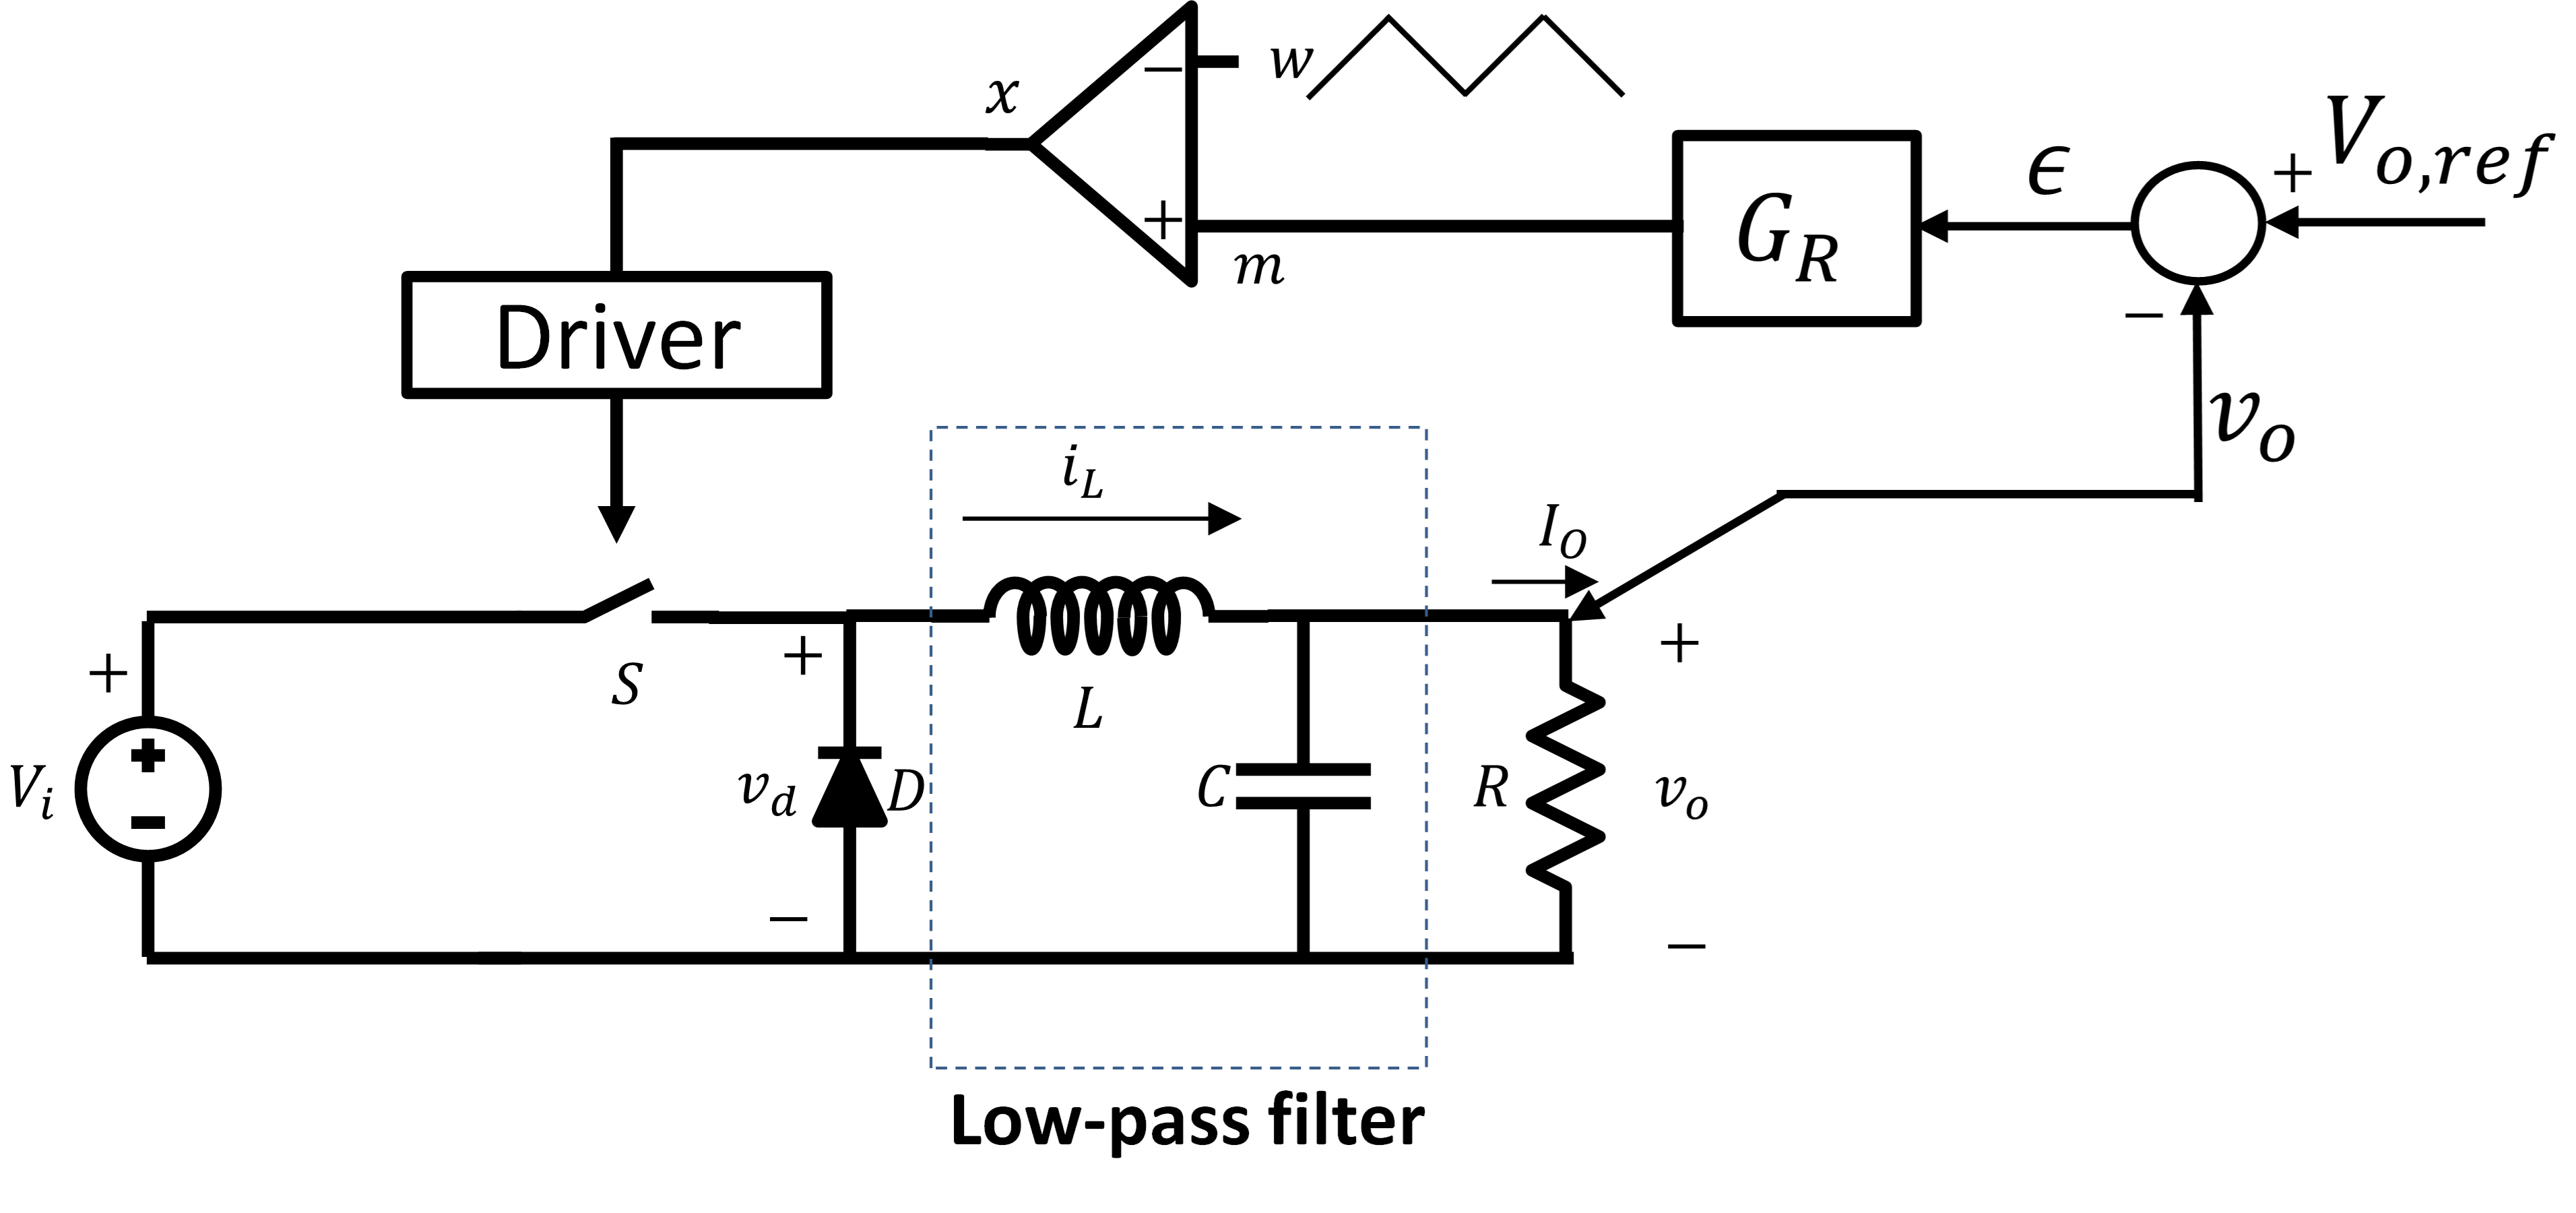
\includegraphics[width=\linewidth]{images/Circuit2.png}
    \caption{Schema circuito}
    \label{fig:Circuit2}
\end{figure}
Il circuito è alimentato dalla tensione duale: $\pm V_{CC}=\pm3V$.\\\\
Il funzionamento per i primi 2 stadi è uguale a quanto detto nel Paragrafo \ref{ch:Spiegazione1}, mentre lo stadio di uscita permette di avere un rendimento migliore di quello ottenuto nell'esperienza precedente. L'efficienza di questo tipo di stadio è dovuta all'attivazione di un solo transistor per semionda. Tuttavia, come si vedrà successivamente, questo circuito ha l'inconveniente di una sensibile distorsione di crossover, dovuta alla soglia di conduzione dei transistor.
\subsection{Assemblaggi e settaggi}
Il circuito in Figura \ref{fig:Circuit2} è stato realizzato modificando direttamente lo schema in classe A (Figura \ref{fig:Circuit1}) con uno stadio in classe B e sostituendo l'integrato MCP6002 con l'integrato TL082CP.\\\\
Lo stadio in classe B push-pull è stato realizzato utilizzando l'accoppiamento di un transistor di potenza NPN $(Q_1)$, codice TIP41CG e un transistor PNP di potenza $(Q_2)$, codice TIP42CG. Le altre componenti sono rimaste invariate dal Primo esperimento\\\\
Il generatore di forma d'onda è stato impostato con il seguente segnale:
\begin{itemize}
    \item Forma d'onda: sinusoidale
    \item Ampiezza iniziale: $100mV$ picco-picco
    \item Frequenza: $330Hz$ (nota Mi)
\end{itemize}
\clearpage
\subsection{Procedura di valutazione e risultati}
Dopo aver acceso l'alimentazione, l'oscilloscopio è stato impostato in modo da visualizzare il segnale di ingresso e il segnale di uscita. Il potenziometro che regola il volume è stato regolato in modo di raggiungere un'ampiezza di $1V_{pp}$ sul segnale di uscita.\\
Si è proseguito a misurare i due segnali con l'oscilloscopio, le cui forme d'onda sono riportare in Figura \ref{fig:scope_9} 
\begin{figure}[H]
    \centering
    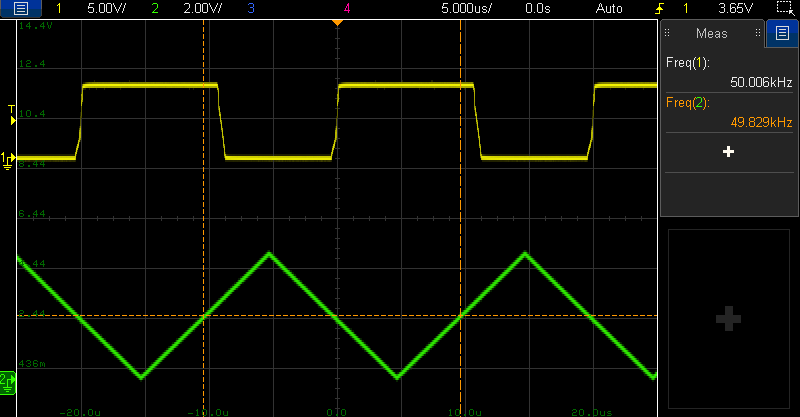
\includegraphics[width=0.7\linewidth]{images/scope_9.png}
    \caption{Segnali di ingresso e uscita dell'amplificatore in classe B}
    \label{fig:scope_9}
\end{figure}
Si è proseguito misurando, attraverso i cursori dell'oscilloscopio, il tempo morto dovuto alla distorsione di crossover.
\begin{equation*}
    \text{Dead time} = 503.125\mu s
\end{equation*}
risultato piùttosto rilevante, considerato che la forma d'onda data in ingresso ha periodo di $T=3\text{ms}$. Si riporta in Figura \ref{fig:scope_11} il dettaglio della distorsione di crossover
\begin{figure}[H]
    \centering
    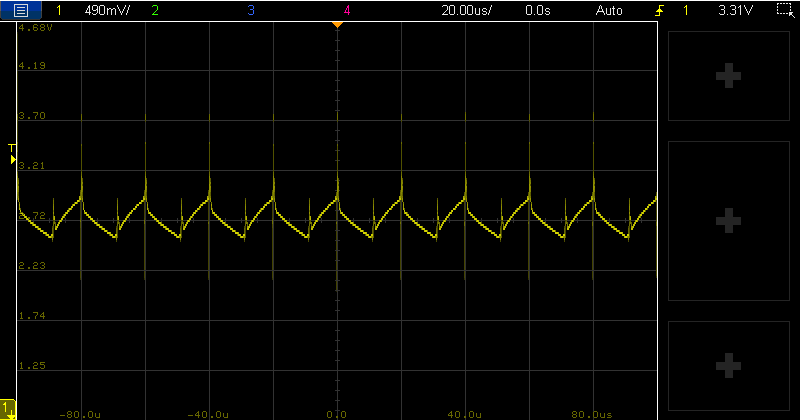
\includegraphics[width=0.7\linewidth]{images/scope_11.png}
    \caption{Dettaglio misurazione distorsione crossover}
    \label{fig:scope_11}
\end{figure}
\subsubsection{Lettore MP3}
Come spiegato nella prima esperienza, si deciso di utilizzare una resistenza di 8$\Omega$ al posto dell'altoparlante, quindi non si è potuto svolgere la prova della riproduzione di una traccia audio. L'obiettivo era quello di sentire l'effetto della distorsione di crossover.
\subsubsection{Commenti}
Le prestazioni di questo amplificatore sono buone, anche se con qualche compromesso. Infatti a livello teorico il rendimento è molto alto, ci sono poce dispersioni di potenza. Come contro, questo circuito ha una distorsione del segnale di uscita decisamente elevata.
    \clearpage
    
    \section[Il futuro della microelettronica]{Il futuro della microelettronica\\ {\small Why new semiconductors like GaN and SiC are much better than silicon for efficient power conversion in energy efficiency applications (electric cars, photovoltaics, etc.)?}}
    L'espansione dei campi di applicazione dei semiconduttori è strettamente collegato all'incremento della complessità dei circuiti e della potenza necessaria per il loro funzionamento.\\
Tuttavia al tempo stesso si sta verificando un  aumento indesiderato dei costi di produzione e funzionamento insieme a una richiesta sempre più stringente di ridurre i gas serra. Questi requisiti contrastanti rende sempre più necessario l'aumento dell'efficienza dei dispositivi elettronici.\\
Un settore in cui questi fattori sono particolarmente sentiti è quello dei convertitori di potenza, estremamente importanti in una vasta gamma di applicazioni. L'efficienza di questi sistemi è molto legata ai transistor utilizzati, che hanno il ruolo di controllare il flusso di corrente verso il carico, le cui caratteristiche spesso determinano dissipazioni non trascurabili di energia.\\Questo ha spinto la ricerca e lo sviluppo di nuove tecnologie a base di silicio e di nuovi materiali ad ampia banda proibita, come il nitruro di gallio (GaN) e il carburo di silicio (SiC).I dispositivi costruiti con questi nuovi materiali offrono notevoli vantaggi, elencati in seguito 
\begin{itemize}
    \item  Funzionamento a \textbf{frequenza più elevata}: i dispositivi in GaN e SiC hanno una maggiore velocità di commutazione che permette di lavorare a frequenze più elevate, consentendo la progettazione di sistemi più efficienti e compatti.
    \item  Funzionamento a \textbf{temperature più elevate}: i dispositivi in GaN e SiC possono funzionare a temperature più elevate rispetto alle controparti in silicio, il che riduce la necessità di grossi sistemi di raffreddamento con un notevole risparmio nei costi e un miglioramento nell'affidabilità dei sistemi elettronici di potenza. 
    \item  Maggiore \textbf{densità di potenza}: i transistor in GaN e SiC hanno una larghezza di banda più ampia consentendo l'utilizzo di campi elettrici più elevati, di conseguenza facilita la progettazione di sistemi elettronici di potenza più piccoli e leggeri.
\end{itemize}
I SiC e i GaN si differenziano nei loro punti di forza. In particolare i Sic sono migliori in applicazioni ad alta temperatura e alta tensione, mentre i GaN in quelle dove la densità di potenza ha priorità assoluta. \\\\ Si può facilmente concludere che questi nuovi materiali presentano vantaggi non trascurabili e che il futuro della microelettronica verterà sull'utilizzo  delle tecnologie dei semiconduttori al Nitruro di Gallio (GaN) e al Carburo di Silicio (SiC), in particolare nei campi di applicazione dove l'efficienza energetica e di spazio sono di primaria importanza.\cite{GaNSiCTexInstru}\cite{InfineonWide}
\printbibliography

\end{document}